\documentclass[11pt]{article}\usepackage[]{graphicx}\usepackage[]{color}
%% maxwidth is the original width if it is less than linewidth
%% otherwise use linewidth (to make sure the graphics do not exceed the margin)
\makeatletter
\def\maxwidth{ %
  \ifdim\Gin@nat@width>\linewidth
    \linewidth
  \else
    \Gin@nat@width
  \fi
}
\makeatother

\definecolor{fgcolor}{rgb}{0.345, 0.345, 0.345}
\newcommand{\hlnum}[1]{\textcolor[rgb]{0.686,0.059,0.569}{#1}}%
\newcommand{\hlstr}[1]{\textcolor[rgb]{0.192,0.494,0.8}{#1}}%
\newcommand{\hlcom}[1]{\textcolor[rgb]{0.678,0.584,0.686}{\textit{#1}}}%
\newcommand{\hlopt}[1]{\textcolor[rgb]{0,0,0}{#1}}%
\newcommand{\hlstd}[1]{\textcolor[rgb]{0.345,0.345,0.345}{#1}}%
\newcommand{\hlkwa}[1]{\textcolor[rgb]{0.161,0.373,0.58}{\textbf{#1}}}%
\newcommand{\hlkwb}[1]{\textcolor[rgb]{0.69,0.353,0.396}{#1}}%
\newcommand{\hlkwc}[1]{\textcolor[rgb]{0.333,0.667,0.333}{#1}}%
\newcommand{\hlkwd}[1]{\textcolor[rgb]{0.737,0.353,0.396}{\textbf{#1}}}%

\usepackage{framed}
\makeatletter
\newenvironment{kframe}{%
 \def\at@end@of@kframe{}%
 \ifinner\ifhmode%
  \def\at@end@of@kframe{\end{minipage}}%
  \begin{minipage}{\columnwidth}%
 \fi\fi%
 \def\FrameCommand##1{\hskip\@totalleftmargin \hskip-\fboxsep
 \colorbox{shadecolor}{##1}\hskip-\fboxsep
     % There is no \\@totalrightmargin, so:
     \hskip-\linewidth \hskip-\@totalleftmargin \hskip\columnwidth}%
 \MakeFramed {\advance\hsize-\width
   \@totalleftmargin\z@ \linewidth\hsize
   \@setminipage}}%
 {\par\unskip\endMakeFramed%
 \at@end@of@kframe}
\makeatother

\definecolor{shadecolor}{rgb}{.97, .97, .97}
\definecolor{messagecolor}{rgb}{0, 0, 0}
\definecolor{warningcolor}{rgb}{1, 0, 1}
\definecolor{errorcolor}{rgb}{1, 0, 0}
\newenvironment{knitrout}{}{} % an empty environment to be redefined in TeX

\usepackage{alltt}
\usepackage{amsmath}
\usepackage{listings}
\usepackage{stmaryrd}
\usepackage{bbm}
\usepackage{amsmath}
\usepackage{mathtools}
\usepackage{pdfpages}
\usepackage{breqn}



\newcount\colveccount
\newcommand*\colvec[1]{
        \global\colveccount#1
        \begin{pmatrix}
        \colvecnext
}
\def\colvecnext#1{
        #1
        \global\advance\colveccount-1
        \ifnum\colveccount>0
                \\
                \expandafter\colvecnext
        \else
                \end{pmatrix}
        \fi
}
\newcommand{\argmin}{\arg\!\min}

\author{Thibault Doutre, Student ID 26980469}
\title{STAT230 HW 9 \\
University of California, Berkeley}
\date{\today}
\IfFileExists{upquote.sty}{\usepackage{upquote}}{}
\begin{document}

\maketitle
\section{Lab 13}
\begin{knitrout}
\definecolor{shadecolor}{rgb}{0.969, 0.969, 0.969}\color{fgcolor}\begin{kframe}
\begin{alltt}
\hlcom{## # LAB 13}

\hlcom{# Import data}
\hlstd{c} \hlkwb{=} \hlkwd{as.matrix}\hlstd{(}\hlkwd{read.table}\hlstd{(}\hlstr{"rindcor.txt"}\hlstd{))}
\hlstd{c} \hlkwb{=} \hlstd{c}\hlopt{+}\hlkwd{t}\hlstd{(c)}
\hlkwd{diag}\hlstd{(c)} \hlkwb{=} \hlnum{1}
\hlstd{c} \hlkwb{=} \hlkwd{as.data.frame}\hlstd{(c)}
\hlkwd{names}\hlstd{(c)} \hlkwb{=} \hlkwd{c}\hlstd{(}\hlstr{"OCC"}\hlstd{,}\hlstr{"RACE"}\hlstd{,}\hlstr{"NOSIB"}\hlstd{,}\hlstr{"FARM"}\hlstd{,}\hlstr{"REGN"}\hlstd{,}
                   \hlstr{"ADOLF"}\hlstd{,}\hlstr{"REL"}\hlstd{,}\hlstr{"YCIG"}\hlstd{,}\hlstr{"FEC"}\hlstd{,}\hlstr{"ED"}\hlstd{,}\hlstr{"EG"}\hlstd{)}
\hlkwd{row.names}\hlstd{(c)} \hlkwb{=} \hlkwd{names}\hlstd{(c)}
\hlstd{c} \hlkwb{=} \hlkwd{as.matrix}\hlstd{(c)}
\hlstd{n} \hlkwb{=} \hlnum{1766}

\hlcom{# Set X, Y and Z}
\hlstd{idx} \hlkwb{=} \hlkwd{c}\hlstd{(}\hlnum{11}\hlstd{,}\hlnum{2}\hlopt{:}\hlnum{8}\hlstd{,}\hlnum{1}\hlstd{)}
\hlstd{idz} \hlkwb{=} \hlkwd{c}\hlstd{(}\hlnum{9}\hlstd{,}\hlnum{2}\hlopt{:}\hlnum{8}\hlstd{,}\hlnum{1}\hlstd{)}
\hlstd{idy} \hlkwb{=} \hlnum{10}

\hlcom{# Perform regression}
\hlstd{Z} \hlkwb{=} \hlstd{c[idz,idz]}\hlopt{*}\hlstd{n}
\hlstd{ZZ_inv} \hlkwb{=} \hlkwd{solve}\hlstd{(Z)}
\hlstd{ZX} \hlkwb{=} \hlstd{c[idz,idx]}\hlopt{*}\hlstd{n}
\hlstd{ZY} \hlkwb{=} \hlstd{c[idz,idy]}\hlopt{*}\hlstd{n}
\hlstd{beta_IVLS} \hlkwb{=} \hlkwd{solve}\hlstd{(}\hlkwd{t}\hlstd{(ZX)} \hlopt \hlstd{ZZ_inv} \hlopt \hlstd{ZX,} \hlkwd{t}\hlstd{(ZX)} \hlopt \hlstd{ZZ_inv} \hlopt \hlstd{ZY)}
\hlstd{beta_IVLS}
\end{alltt}
\begin{lstlisting}[basicstyle=\ttfamily,breaklines=true]
##              [,1]
## EG     0.14727108
## RACE  -0.07652004
## NOSIB -0.21655055
## FARM  -0.02330998
## REGN  -0.10928188
## ADOLF -0.14559186
## REL   -0.09242772
## YCIG  -0.12776409
## OCC    0.24837554
\end{lstlisting}
\begin{alltt}
\hlcom{# Standard errors}
\hlstd{XX} \hlkwb{=} \hlstd{c[idx,idx]}\hlopt{*}\hlstd{n}
\hlstd{YX} \hlkwb{=} \hlstd{c[idy,idx]}\hlopt{*}\hlstd{n}
\hlstd{YY} \hlkwb{=} \hlstd{c[idy,idy]}\hlopt{*}\hlstd{n}
\hlstd{e2} \hlkwb{=} \hlstd{YY} \hlopt{+} \hlkwd{t}\hlstd{(beta_IVLS)} \hlopt \hlstd{XX} \hlopt \hlstd{beta_IVLS} \hlopt{-} \hlnum{2} \hlopt{*} \hlstd{(YX} \hlopt \hlstd{beta_IVLS)}
\hlstd{sigma_hat} \hlkwb{=} \hlkwd{sqrt}\hlstd{(}\hlkwd{as.numeric}\hlstd{(e2)}\hlopt{/}\hlstd{(n}\hlopt{-}\hlnum{9}\hlstd{))}
\hlstd{sigma_hat}\hlopt{^}\hlnum{2}
\end{alltt}
\begin{lstlisting}[basicstyle=\ttfamily,breaklines=true]
## [1] 0.6745362
\end{lstlisting}
\begin{alltt}
\hlstd{cov_hat} \hlkwb{=} \hlstd{(sigma_hat}\hlopt{^}\hlnum{2}\hlstd{)}\hlopt{*}\hlkwd{solve}\hlstd{(}\hlkwd{t}\hlstd{(ZX)} \hlopt \hlstd{ZZ_inv} \hlopt \hlstd{ZX)}

\hlstd{se_hat} \hlkwb{=} \hlkwd{sqrt}\hlstd{(}\hlkwd{diag}\hlstd{(cov_hat))}
\hlstd{se_hat}
\end{alltt}
\begin{lstlisting}[basicstyle=\ttfamily,breaklines=true]
##         EG       RACE      NOSIB       FARM       REGN 
## 0.09253546 0.02488338 0.02109963 0.02181783 0.02379165 
##      ADOLF        REL       YCIG        OCC 
## 0.02460040 0.02102358 0.02277556 0.02468539
\end{lstlisting}
\end{kframe}
\end{knitrout}
The coefficients in Rindfuss et al. are slightly different, probably because of the rounding errors in the correlation matrix.

\section{Simulation IVLS vs OLS}
\begin{knitrout}
\definecolor{shadecolor}{rgb}{0.969, 0.969, 0.969}\color{fgcolor}\begin{kframe}
\begin{alltt}
\hlcom{## # IVLS Simulation}

\hlcom{# Function to generate delta and eps}
\hlstd{generate_delta_eps} \hlkwb{=} \hlkwa{function}\hlstd{(}\hlkwc{n}\hlstd{)\{}
  \hlcom{# Define parameters}
  \hlstd{rho} \hlkwb{=} \hlnum{0.3}
  \hlstd{mu1}\hlkwb{=}\hlnum{0}\hlstd{; s1}\hlkwb{=}\hlnum{1}\hlstd{; mu2}\hlkwb{=}\hlnum{0}\hlstd{; s2}\hlkwb{=}\hlnum{1}

  \hlcom{# Define X, Y and Z with the bivariate normal relationship}
  \hlstd{X} \hlkwb{=} \hlkwd{rnorm}\hlstd{(n)}
  \hlstd{Z} \hlkwb{=} \hlkwd{rnorm}\hlstd{(n)}
  \hlstd{eps} \hlkwb{=} \hlkwd{sqrt}\hlstd{(}\hlnum{1}\hlopt{-}\hlstd{rho}\hlopt{^}\hlnum{2}\hlstd{)} \hlopt{*} \hlstd{Z}
  \hlstd{Y} \hlkwb{=} \hlstd{rho} \hlopt{*} \hlstd{X} \hlopt{+} \hlstd{eps}

  \hlcom{# Adjust means and variances}
  \hlstd{Y} \hlkwb{=} \hlstd{(Y}\hlopt{-}\hlkwd{mean}\hlstd{(Y))}\hlopt{/}\hlkwd{sd}\hlstd{(Y)}\hlopt{*}\hlstd{s2}\hlopt{+}\hlstd{mu2}
  \hlstd{X} \hlkwb{=} \hlstd{(X}\hlopt{-}\hlkwd{mean}\hlstd{(X))}\hlopt{/}\hlkwd{sd}\hlstd{(X)}\hlopt{*}\hlstd{s1}\hlopt{+}\hlstd{mu1}

  \hlcom{# Adjust rho by transforming Y}
  \hlstd{rho_hat} \hlkwb{=} \hlkwd{cor}\hlstd{(X,Y)}
  \hlstd{a} \hlkwb{=} \hlstd{s1}\hlopt{^}\hlnum{4}\hlopt{*}\hlstd{(rho}\hlopt{^}\hlnum{2}\hlopt{-}\hlnum{1}\hlstd{)}
  \hlstd{b} \hlkwb{=} \hlnum{2}\hlopt{*}\hlstd{rho_hat}\hlopt{*}\hlstd{s1}\hlopt{^}\hlnum{3}\hlopt{*}\hlstd{s2}\hlopt{*}\hlstd{(rho}\hlopt{^}\hlnum{2}\hlopt{-}\hlnum{1}\hlstd{)}
  \hlstd{c} \hlkwb{=} \hlstd{(rho}\hlopt{^}\hlnum{2}\hlopt{-}\hlstd{rho_hat}\hlopt{^}\hlnum{2}\hlstd{)}\hlopt{*}\hlstd{s2}\hlopt{^}\hlnum{2}\hlopt{*}\hlstd{s1}\hlopt{^}\hlnum{2}
  \hlstd{delta} \hlkwb{=} \hlstd{b}\hlopt{^}\hlnum{2}\hlopt{-}\hlnum{4}\hlopt{*}\hlstd{a}\hlopt{*}\hlstd{c}
  \hlstd{correction} \hlkwb{=} \hlstd{(}\hlopt{-}\hlstd{b}\hlopt{-}\hlkwd{sqrt}\hlstd{(delta))}\hlopt{/}\hlstd{(}\hlnum{2}\hlopt{*}\hlstd{a)}
  \hlstd{Y}\hlkwb{=}\hlstd{Y}\hlopt{+}\hlstd{correction}\hlopt{*}\hlstd{X}

  \hlcom{# Adjust means and variances}
  \hlstd{Y} \hlkwb{=} \hlstd{(Y}\hlopt{-}\hlkwd{mean}\hlstd{(Y))}\hlopt{/}\hlkwd{sd}\hlstd{(Y)}\hlopt{*}\hlstd{s2}\hlopt{+}\hlstd{mu2}
  \hlstd{X} \hlkwb{=} \hlstd{(X}\hlopt{-}\hlkwd{mean}\hlstd{(X))}\hlopt{/}\hlkwd{sd}\hlstd{(X)}\hlopt{*}\hlstd{s1}\hlopt{+}\hlstd{mu1}

  \hlkwd{return}\hlstd{(}\hlkwd{cbind}\hlstd{(X,Y))}
\hlstd{\}}

\hlcom{# Simulate B betas for IVLS and OLS}
\hlstd{simulation_betas} \hlkwb{=} \hlkwa{function}\hlstd{(}\hlkwc{n}\hlstd{,}\hlkwc{C}\hlstd{,}\hlkwc{B}\hlstd{)\{}
  \hlstd{beta_OLS_values} \hlkwb{=} \hlkwd{c}\hlstd{()}
  \hlstd{beta_IVLS_values} \hlkwb{=} \hlkwd{c}\hlstd{()}
  \hlkwa{for} \hlstd{(i} \hlkwa{in} \hlnum{1}\hlopt{:}\hlstd{B)\{}
    \hlcom{# True beta}
    \hlstd{beta} \hlkwb{=} \hlnum{1}
    \hlcom{# Generate Z}
    \hlstd{Z} \hlkwb{=} \hlkwd{rnorm}\hlstd{(n)}
    \hlcom{# Generate delta and eps}
    \hlstd{delta_eps} \hlkwb{=} \hlkwd{generate_delta_eps}\hlstd{(n)}
    \hlstd{delta} \hlkwb{=} \hlstd{delta_eps[,}\hlnum{1}\hlstd{]}
    \hlstd{eps} \hlkwb{=} \hlstd{delta_eps[,}\hlnum{2}\hlstd{]}
    \hlcom{# Generate X}
    \hlstd{X} \hlkwb{=} \hlstd{C}\hlopt{*}\hlstd{Z}\hlopt{+}\hlstd{delta}
    \hlcom{# Generate Y}
    \hlstd{Y} \hlkwb{=} \hlstd{X}\hlopt{*}\hlstd{beta}\hlopt{+}\hlstd{eps}
    \hlcom{# Estimates of beta}
    \hlstd{beta_OLS} \hlkwb{=} \hlkwd{solve}\hlstd{(}\hlkwd{t}\hlstd{(X)}\hlopt\hlstd{X)} \hlopt \hlkwd{t}\hlstd{(X)} \hlopt \hlstd{Y}
    \hlstd{beta_IVLS} \hlkwb{=} \hlkwd{solve}\hlstd{(}\hlkwd{t}\hlstd{(X)}\hlopt\hlstd{Z} \hlopt \hlkwd{solve}\hlstd{(}\hlkwd{t}\hlstd{(Z)}\hlopt\hlstd{Z)} \hlopt \hlkwd{t}\hlstd{(Z)}\hlopt\hlstd{X)} \hlopt
      \hlkwd{t}\hlstd{(X)}\hlopt\hlstd{Z} \hlopt \hlkwd{solve}\hlstd{(}\hlkwd{t}\hlstd{(Z)}\hlopt\hlstd{Z)} \hlopt \hlkwd{t}\hlstd{(Z)}\hlopt\hlstd{Y}
    \hlstd{beta_OLS_values} \hlkwb{=}\hlkwd{c}\hlstd{(beta_OLS_values,beta_OLS)}
    \hlstd{beta_IVLS_values}\hlkwb{=}\hlkwd{c}\hlstd{(beta_IVLS_values,beta_IVLS)}
  \hlstd{\}}
  \hlkwd{list}\hlstd{(}\hlkwc{OLS}\hlstd{=beta_OLS_values,}\hlkwc{IVLS}\hlstd{=beta_IVLS_values)}
\hlstd{\}}

\hlstd{output_results} \hlkwb{=} \hlkwa{function}\hlstd{(}\hlkwc{C}\hlstd{,}\hlkwc{n}\hlstd{,}\hlkwc{B}\hlstd{)\{}
  \hlstd{sim} \hlkwb{=} \hlkwd{simulation_betas}\hlstd{(n,C,B)}
  \hlstd{sim_OLS} \hlkwb{=} \hlstd{sim}\hlopt{$}\hlstd{OLS}
  \hlstd{sim_IVLS} \hlkwb{=} \hlstd{sim}\hlopt{$}\hlstd{IVLS}
  \hlstd{mse_OLS} \hlkwb{=} \hlstd{(sim_OLS}\hlopt{-}\hlnum{1}\hlstd{)}\hlopt{^}\hlnum{2}
  \hlstd{mse_IVLS} \hlkwb{=} \hlstd{(sim_IVLS}\hlopt{-}\hlnum{1}\hlstd{)}\hlopt{^}\hlnum{2}

  \hlkwd{par}\hlstd{(}\hlkwc{mfrow} \hlstd{=} \hlkwd{c}\hlstd{(}\hlnum{2}\hlstd{,}\hlnum{1}\hlstd{))}
  \hlkwd{hist}\hlstd{(mse_OLS,} \hlkwc{main} \hlstd{=} \hlstr{"MSE OLS"}\hlstd{)}
  \hlkwd{hist}\hlstd{(mse_IVLS,} \hlkwc{main} \hlstd{=} \hlstr{"MSE IVLS"}\hlstd{)}
  \hlkwd{par}\hlstd{(}\hlkwc{mfrow} \hlstd{=} \hlkwd{c}\hlstd{(}\hlnum{1}\hlstd{,}\hlnum{1}\hlstd{))}

  \hlkwd{print}\hlstd{(}\hlstr{'Summary OLS'}\hlstd{)}
  \hlkwd{print}\hlstd{(}\hlkwd{summary}\hlstd{(mse_OLS))}
  \hlkwd{print}\hlstd{(}\hlstr{'Summary IVLS'}\hlstd{)}
  \hlkwd{print}\hlstd{(}\hlkwd{summary}\hlstd{(mse_IVLS))}
\hlstd{\}}
\end{alltt}
\end{kframe}
\end{knitrout}

\begin{knitrout}
\definecolor{shadecolor}{rgb}{0.969, 0.969, 0.969}\color{fgcolor}\begin{kframe}
\begin{alltt}
\hlstd{B}\hlkwb{=}\hlnum{1000}
\hlcom{# Simumation 1}
\hlstd{C}\hlkwb{=}\hlnum{.1}
\hlstd{n}\hlkwb{=}\hlnum{10}
\hlkwd{output_results}\hlstd{(C,n,B)}
\end{alltt}
\end{kframe}
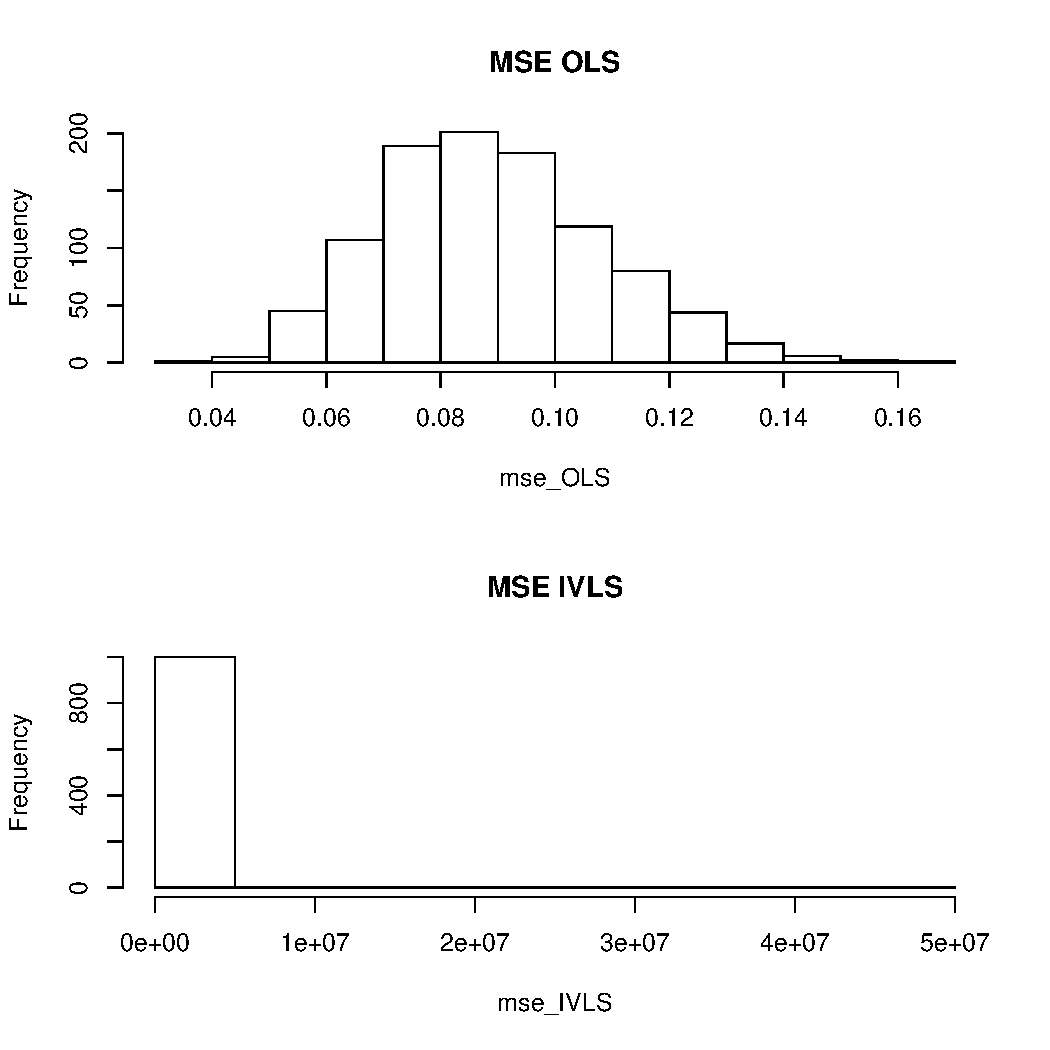
\includegraphics[width=\maxwidth]{figure/unnamed-chunk-4-1} 
\begin{kframe}\begin{lstlisting}[basicstyle=\ttfamily,breaklines=true]
## [1] "Summary OLS"
##    Min. 1st Qu.  Median    Mean 3rd Qu.    Max. 
## 0.03759 0.07574 0.08732 0.08924 0.10170 0.16220 
## [1] "Summary IVLS"
##     Min.  1st Qu.   Median     Mean  3rd Qu.     Max. 
##        0        0        1    48670        5 48050000
\end{lstlisting}
\end{kframe}
\end{knitrout}
OLS performs better here.

\begin{knitrout}
\definecolor{shadecolor}{rgb}{0.969, 0.969, 0.969}\color{fgcolor}\begin{kframe}
\begin{alltt}
\hlcom{# Simumation 2}
\hlstd{C}\hlkwb{=}\hlnum{.5}
\hlstd{n}\hlkwb{=}\hlnum{10}
\hlkwd{output_results}\hlstd{(C,n,B)}
\end{alltt}
\end{kframe}
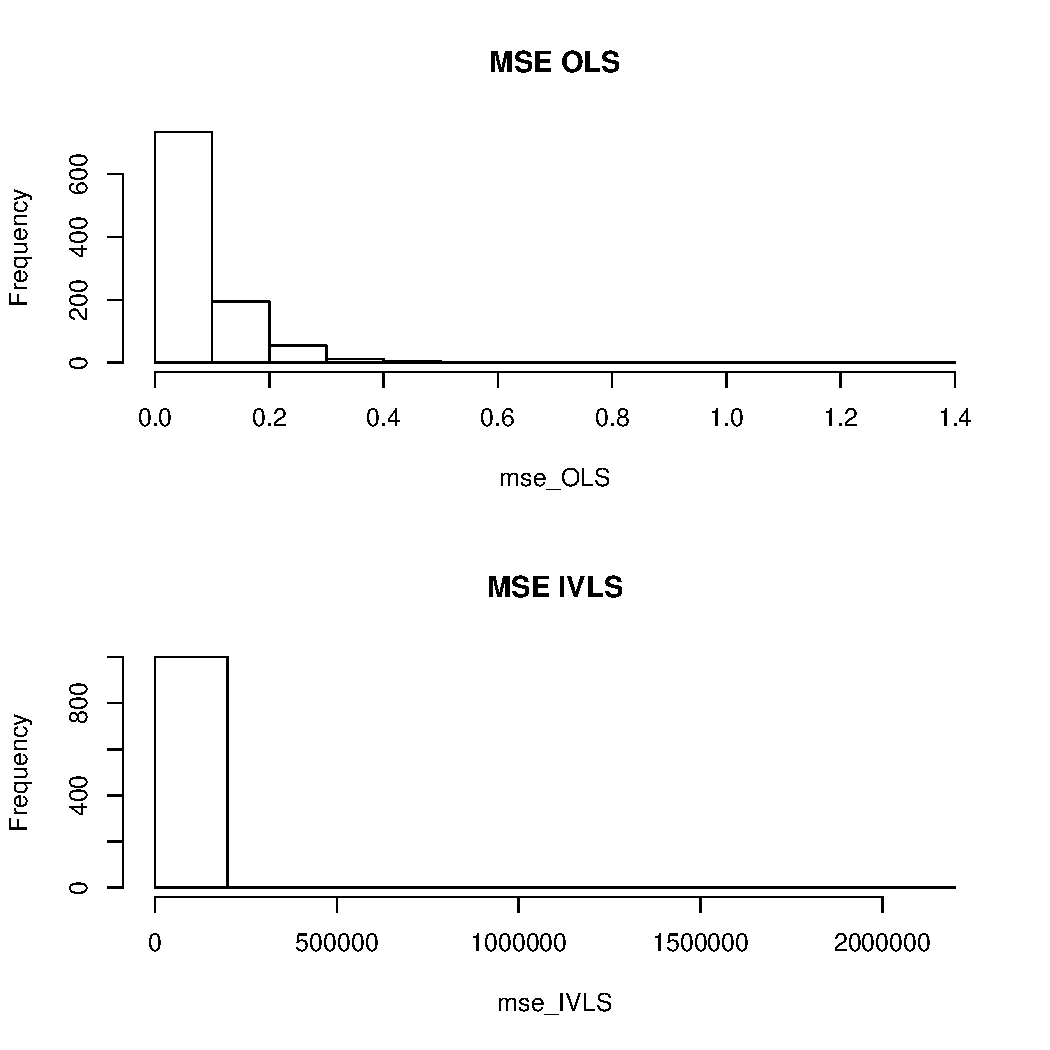
\includegraphics[width=\maxwidth]{figure/unnamed-chunk-5-1} 
\begin{kframe}\begin{lstlisting}[basicstyle=\ttfamily,breaklines=true]
## [1] "Summary OLS"
##    Min. 1st Qu.  Median    Mean 3rd Qu.    Max. 
## 0.00000 0.02284 0.05537 0.07795 0.10460 1.33500 
## [1] "Summary IVLS"
##      Min.   1st Qu.    Median      Mean   3rd Qu.      Max. 
##       0.0       0.0       0.2    2153.0       0.9 2028000.0
\end{lstlisting}
\end{kframe}
\end{knitrout}
OLS performs better here.

\begin{knitrout}
\definecolor{shadecolor}{rgb}{0.969, 0.969, 0.969}\color{fgcolor}\begin{kframe}
\begin{alltt}
\hlcom{# Simumation 3}
\hlstd{C}\hlkwb{=}\hlnum{.1}
\hlstd{n}\hlkwb{=}\hlnum{1000}
\hlkwd{output_results}\hlstd{(C,n,B)}
\end{alltt}
\end{kframe}
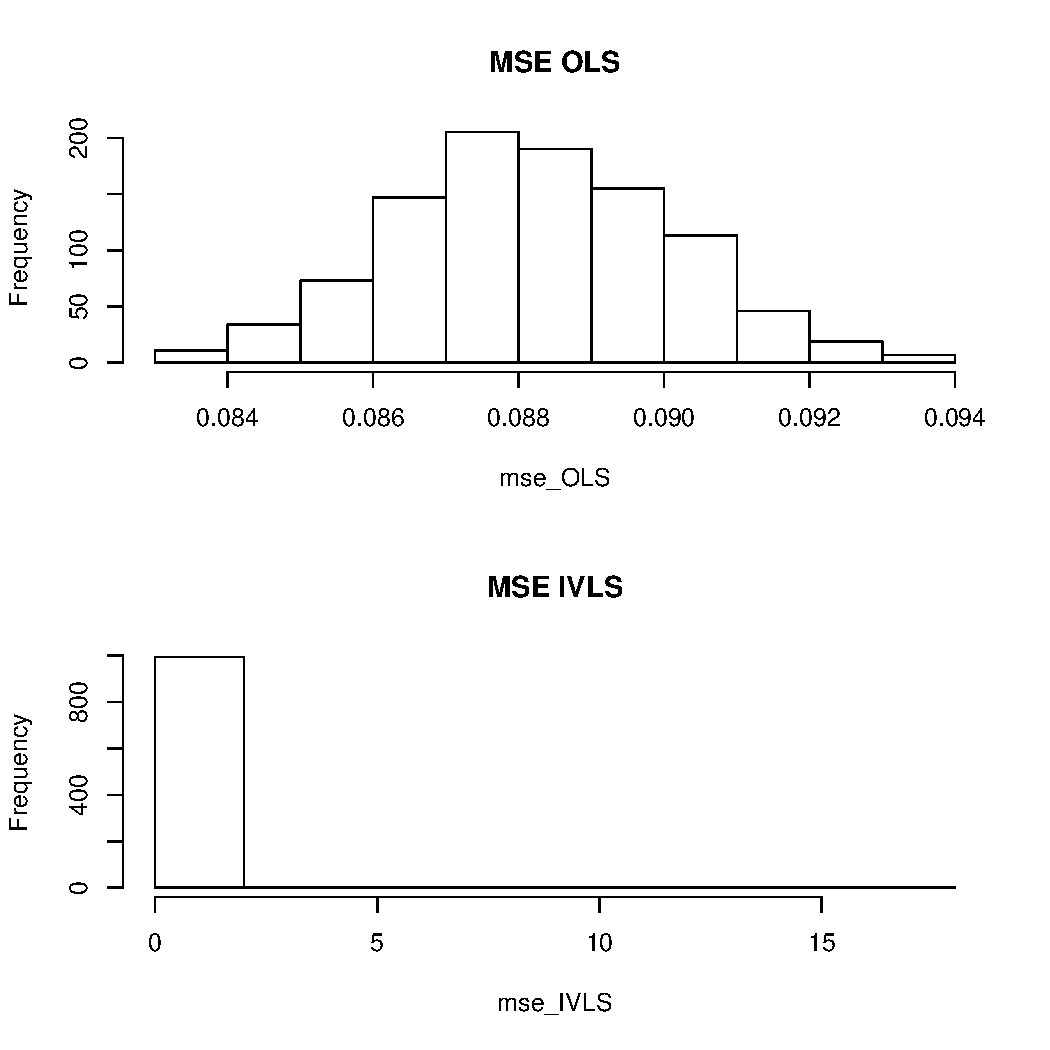
\includegraphics[width=\maxwidth]{figure/unnamed-chunk-6-1} 
\begin{kframe}\begin{lstlisting}[basicstyle=\ttfamily,breaklines=true]
## [1] "Summary OLS"
##    Min. 1st Qu.  Median    Mean 3rd Qu.    Max. 
## 0.08342 0.08690 0.08814 0.08821 0.08955 0.09387 
## [1] "Summary IVLS"
##     Min.  1st Qu.   Median     Mean  3rd Qu.     Max. 
##  0.00000  0.01190  0.05777  0.17740  0.16030 16.54000
\end{lstlisting}
\end{kframe}
\end{knitrout}
OLS performs better here.

\begin{knitrout}
\definecolor{shadecolor}{rgb}{0.969, 0.969, 0.969}\color{fgcolor}\begin{kframe}
\begin{alltt}
\hlcom{# Simumation 4}
\hlstd{C}\hlkwb{=}\hlnum{.5}
\hlstd{n}\hlkwb{=}\hlnum{1000}
\hlkwd{output_results}\hlstd{(C,n,B)}
\end{alltt}
\end{kframe}
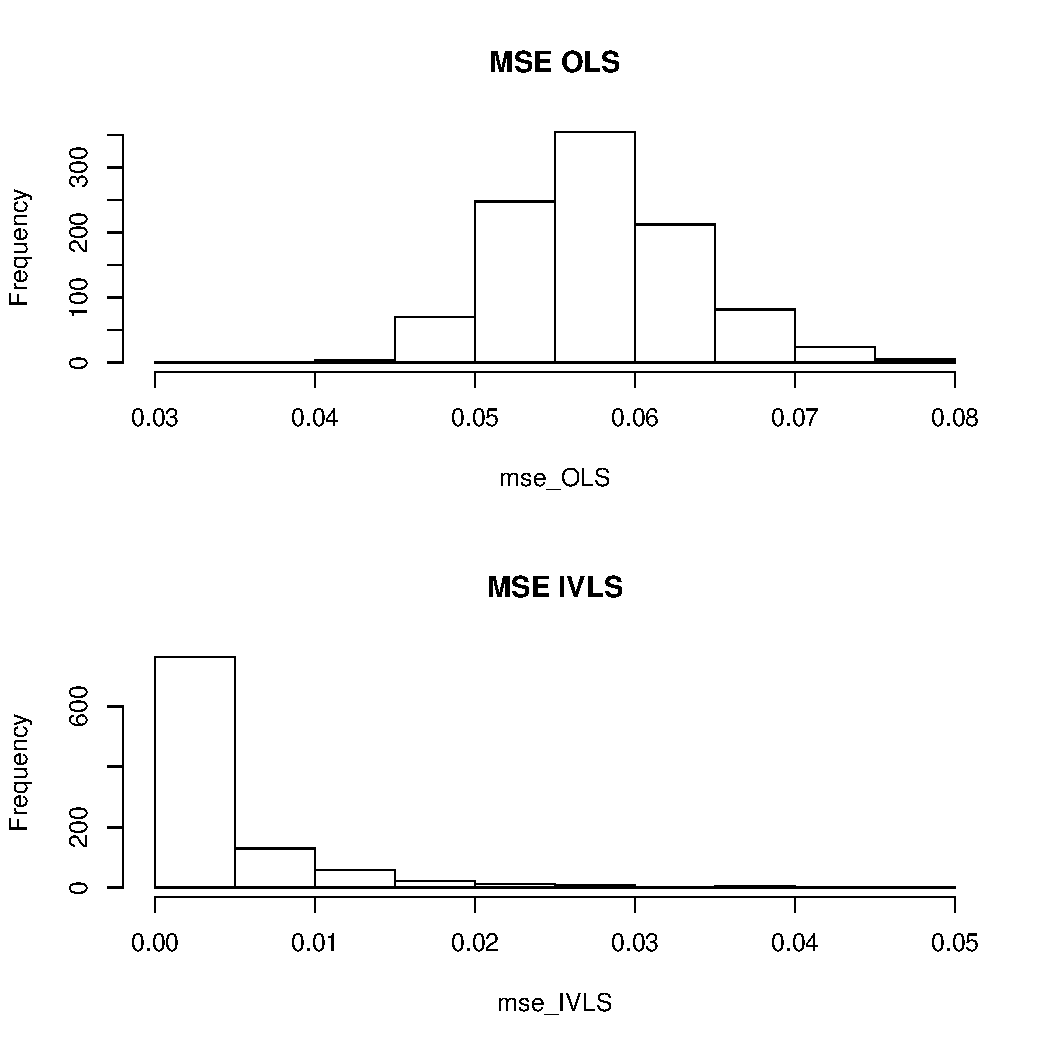
\includegraphics[width=\maxwidth]{figure/unnamed-chunk-7-1} 
\begin{kframe}\begin{lstlisting}[basicstyle=\ttfamily,breaklines=true]
## [1] "Summary OLS"
##    Min. 1st Qu.  Median    Mean 3rd Qu.    Max. 
## 0.03487 0.05372 0.05750 0.05777 0.06144 0.07776 
## [1] "Summary IVLS"
##      Min.   1st Qu.    Median      Mean   3rd Qu.      Max. 
## 1.000e-08 3.922e-04 1.600e-03 3.772e-03 4.813e-03 4.592e-02
\end{lstlisting}
\end{kframe}
\end{knitrout}
IVLS performs better here.
\\
IVLS performs better as we increase both $C$ and $n$. We have the following equation: (simultaneity bias)^2 + OLS variance $<$ (small-sample bias)^2 + IVLS variance. Thus, sometimes OLS has a smaller mean squared error than IVLS (low $C$ or low $n$).

\end{document}









